%---Include Befehle-------------------------------------------------------------------
\documentclass[a4paper]{article}
\usepackage{ngerman, amsmath, amssymb, bbm, array, tabularx}
\usepackage[T1]{fontenc}
\usepackage[utf8]{inputenc} 		% Kodierung
\usepackage[ngerman]{babel} 		% Sprache
\usepackage{textcomp}       		% Zusätzliche Symbolzeichen 
\setlength{\parskip}{1.5ex plus0.5ex minus0.2ex} 
\setlength{\parindent}{0cm}
\usepackage[]{graphicx}   			% initialisierung von Graphiken
\usepackage{xcolor}					% init von Farbe
\usepackage{tabularx}				% verbesserte Tabs

%---Seitenränder einstellen-----------------------------------------------------------
\usepackage[left=30mm,right=25mm,top=25mm,bottom=25mm]{geometry}

%---Kopf- und Fusszeile---------------------------------------------------------------
\usepackage{fancyhdr}
\pagestyle{fancy}
\fancyhf{}
\lhead{{\footnotesize HTW Berlin}} 				% linke Seite Kopfzeile, Größe wie eine Fußnote
\chead{} 										% Mitte Kopf - leer
\rhead{{\footnotesize SWE - Belegarbeit GIT}} 	% rechte Seite Kopfzeile
\lfoot{{\footnotesize F. Goerge, S. Ede,\\ R. Peters, J. Meise}} %linke Seite Fußnote
\cfoot{} 										% Mitte Fußnote leer
\rfoot{\thepage} 								% Rechte Fußnote Seitenzahl
\renewcommand{\headrulewidth}{0.2pt}    		% Größe Kopf/Fußzeile?
\renewcommand{\footrulewidth}{0.2pt}

%---Glossar---------------------------------------------------------------------------
\usepackage[urlcolor=blue,colorlinks=true,linkcolor=blue]{hyperref} %Farbe der Links in blau
\usepackage[toc,style=treenoname,order=word,subentrycounter]{glossaries} 
\makeglossaries

%---Glossareinträge-------------------------------------------------------------------
%Glossar update Info. -> Benutzer/in -> Eigene Befehle -> Eigene Befehle editieren
% --> makeindex -s %.ist -t %.glg -o %.gls %.glo
% und unter -> Option -> Texmaker konfigurieren -> Makeindex Verweis aktualisieren!

\newglossaryentry{merge}		{name=Merge		,description={engl. zusammenführen - Vereinigung von Branches}}
\newglossaryentry{Repository}	{name=Repository,description={engl. Lager, Depot - Repositorium enthält die Geschichte eines Projekts. Jeder Nutzer hat ein eigenes Repository mit der gesamten Geschichte}}
\newglossaryentry{Clone} 		{name=Clone		,description={engl. kopieren - Ein entferntes Repository wird auf einen lokalen Rechner übertragen}}
\newglossaryentry{Branch}		{name=Branch	,description={engl. Zweig - Ein Branch ist ein Entwicklungszweig in der Geschichte}}
\newglossaryentry{Switch}		{name=Switch	,description={engl. wechseln - Switch ermöglicht das Wechseln auf einen anderen Branch (arbeitet man z.B. auf einem seperaten Branch, könnte man mit Switch zurück zum Master Branch wechseln)}}
\newglossaryentry{pull}			{name=Pull		,description={engl. ziehen - Pull lädt alle Änderungen vom externen Repository}}
\newglossaryentry{commit}		{name=Commit	,description={engl. übergeben - Mit diesem Befehl werden lokale Änderungen im lokalen Repository gespeichert}}
\newglossaryentry{Changeset}		{name=Changeset	,description={In einem Changeset werden mehrere Änderungen zu einer Einheit zusammengefasst}}
\newglossaryentry{push}		{name=Push		,description={engl. anschieben - Dieser Befehl überträgt die lokalen Änderungen auf den Server}}
%-------------------------------------------------------------------------------------

\begin{document}

%---Deckblatt-------------------------------------------------------------------------
\title{\textbf{{\Huge { Belegarbeit GIT \vspace{2cm}} 

\includegraphics[width=\textwidth]{git-logo.png}	% einfügen von Bildern
\vspace{2cm} }}}
\author{Fabian Goerge \\  Sami Ede  \\ Richard Peters \\ Jens Meise}
\date{\today}
\maketitle
\thispagestyle{empty} 								% Keine Seitenzahl auf dem Deckblatt 

%------------------------------------------------------------------------------------

\newpage

%---Inhaltsverzeichnis wird erzeugt--------------------------------------------------
\setcounter{page}{1} 								% Inhaltsverzeichnis startet mit der Seitenzahl 1 
\tableofcontents									% Inhaltsverzeichnis wird erzeugt

%------------------------------------------------------------------------------------

\newpage

%---Erster Punkt--------------------------------------------------------------------
\section{\underline{Einführung und Ziel der Arbeit}} 	% Section erstellt automatisch den jeweiligen Punkt. Das erste Section erstellt Punkt 1, das 2te Punkt 1 etc.

\subsection{Einführung} 								% Subsection erstellt automatisch Unterpunkte

Git ist ein freies Versionsverwaltungssystem, dass von Linus Torvald entwickelt wurde.
(Das zu der Zeit existierende Versionsverwaltungssystem BitKeeper war aus Lizenzgründen nicht mehr für das Linuxentwicklerteam zugänglich, und so entschied sich Torvald dafür, ein eigenes System zu schreiben.) \\
Ein Versionsverwaltungssystem verfolgt Änderungen in Dokumenten oder Dateien und speichert die durch die Änderungen entstehenden Versionen in einem Verzeichnis so ab, dass sie mit einem Zeitstempel und einer Benuzerkennung versehen werden und später wieder hergestellt werden können. Git bietet weiterhin die Möglichkeit sich eigene \gls{Branch}es zu erstellen, so dass man unabhängig vom "Hauptstrang" arbeiten kann, ohne in Gefahr zu laufen, wichtige Teile des Codes unbeabsichtlich zu zerstören, um so zum Beispiel Portierungen einer Applikation auf andere Betriebssysteme zu entwickeln. \\
Git speichert außerdem alle Dateien lokal, so dass auch ohne Internetverbindung gearbeitet werden kann, die Zusammenführung (\gls{merge}) der Branches muss dann zu einem späteren Zeitpunkt stattfinden. Jeder Benutzer verfügt also über eine komplette Kopie des \gls{Repository}. \\
Die Speicherung der Versionsgeschichte erfolgt so, dass der Name einer beliebigen Revision auf der vollständigen Geschichte basiert, die zu dieser Version geführt hat, so dass es nicht möglich ist, die Versionsgeschichte nachträglich zu ändern. Diese Funktion ermöglicht auch, bestimmte Versionen gesondert digital zu signieren, um z.B. den Zustand zum Zeitpunkt des Erscheinens einer neuen Version besonders zu kennzeichnen. \\
Ein weiterer Vorteil von Git ist zudem eine große Vielfalt von Möglichkeiten zum Austausch zwischen Repositories; Git unterstützt eine Vielzahl von Protokollen zum Dateiaustausch, darunter auch ein eigenes, sehr effizientes (git://).\\


\subsection{Ziel}
	Das Ziel dieses Projektes, ist die Modellierung von Git, die Darstellung und Rekonstruktion einer Software über Diagramme, sowie die Auseinandersetzung mit den verschiedenen Modellierungsarten. \\
	Dafür werden wir uns zunächst mit einem Use-Case-Modell beschäftigen und dieses anschließend in einigen Use-Case-Szenarien elaborieren. \\
	Außerdem wird ein Domänenmodell dargestellt, sowie einige ausgewählte Zustandsdiagramme.\\
	Abschließend erläutern wir einige Erfahrungen aus der Teamarbeit und eine Schlussbetrachtung.
\newpage												% Seitenumbruch
\section{\underline{Textuelle Beschreibung}}

Git ist eine freie Software zur verteilten Versionsverwaltung von Dateien. Git hilft, wenn mehrere Programmierer an einem Projekt arbeiten, indem es verschiedene Features vereint:

  \begin{itemize} 										% Aufzählungen
     
\item Git ermöglicht eine nicht-lineare Entwicklung; das heißt, es ist möglich, an verschiedenen „Positionen“ des Quelltextes zu arbeiten, und diese im Nachhinein automatisch zu vereinen („mergen“). %Jeder Backslash ist ein Bulletpoint
\item des Weiteren bietet Git die Möglichkeit eines lokalen Arbeitens. Jeder User besitzt eine lokale Kopie des kompletten Repositories (inklusive der Versionsgeschichte), so dass auch ohne Anbindung in ein Netzwerk gearbeitet werden kann. Dies ermöglicht sehr schnelles Arbeiten!
Dies bedeutet auch gleichzeitig Multi-Backups! Jeder User speichert die komplette Versionsgeschichte!
\item Mehrere Möglichkeiten, Repositories abzugleichen; Git besitzt ein eigenes Protokoll, und unterstützt unter anderem http, https, ftp und rsync Übertragungen.
\item Versionsgeschichte wird kryptografisch gesichert, so dass es nicht möglich ist, Änderungen an der Versionsgeschichte vorzunehmen, ohne dass sich der Name der Revision ändert.

    \end{itemize} 										% Aufzählung beendet

Außerdem bietet Git ein Webinterface.

\section{\underline{Modellierung}}

\subsection{Use-Case-Modell}

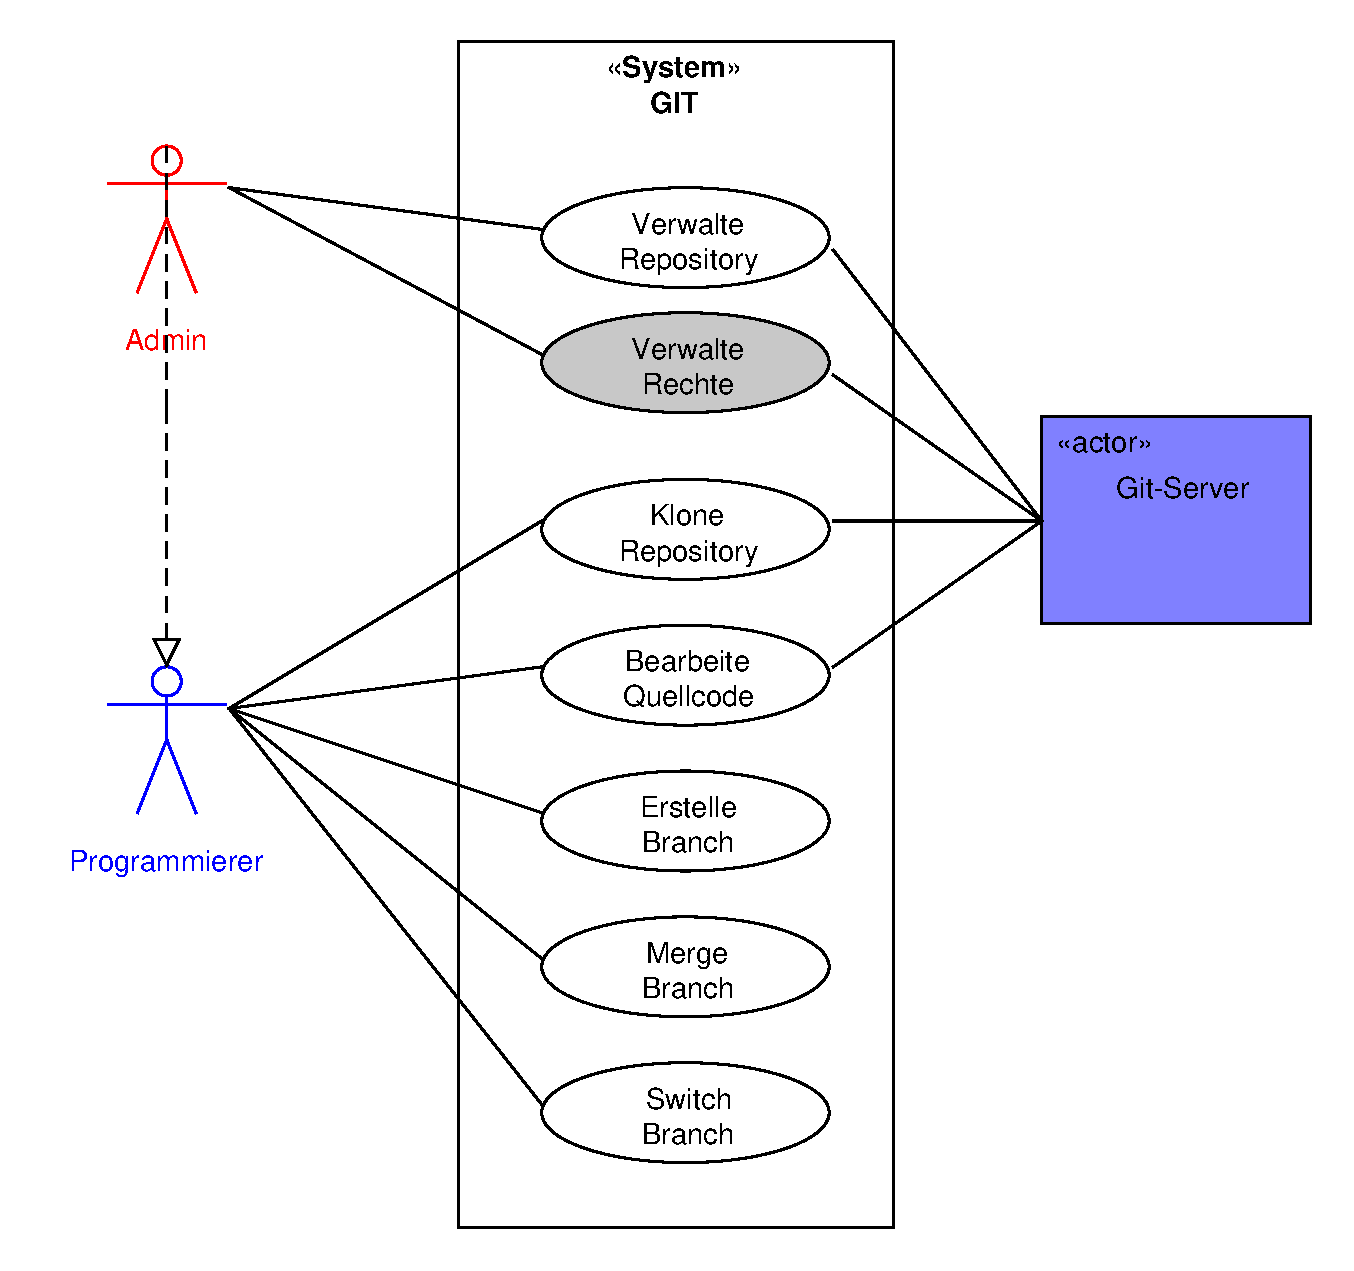
\includegraphics[width=15cm]{Use-Case-Modell.pdf}	

Dieses Use-Cases repräsentieren die Interaktion zwischen dem Programmierer (\textit{Aktor}) und dem Git-System (\textit{Subjekt})\\  							% Textit = Textitalian = kursiv
\\ 														% Absatz
Der Programmierer benutzt das Git-System um ein bestimmtes Ziel zu erreichen. 
Der Git-Server (\textit{Sekundäre Aktor}) wird genutzt um mit den lokalen GIT Instanzen synchronisiert zu werden.\\
\\
Der Programmierer repräsentiert eine Personengruppe. An einem Projekt können beliebig viele Programmierer beteiligt seien.  
Der Admin erbt alle Fähigkeiten von dem Programmierer. Demnach kann der Admin auch alle anderen Interaktionen ausüben.  \\
\\
Im Use-Case sind die Möglichkeiten, verwalte Repository, \gls{Clone} Repository, bearbeite Quellcode, erstelle Branch, Merge Branch und \gls{Switch} Branch aufgeführt.\\\\Optional besteht die Möglichkeit für den Admin die Rechte mit Hilfe der Betriebssystemverwaltung über ein Skript in GIT zu integrieren.\\
\\
Eine detaillierte Beschreibung der Abläufe folgt in den Use-Case-Szenarien. 

\newpage	
\subsubsection{Use-Case-Szenarien (Storys)}

	
\begin{tabularx}{\textwidth}{lX}
\\
\textbf{Use Case:} & Clone Repository \\
\textbf{Kurzbeschreibung:}& Der Programmierer kopiert sämtliche Daten des Repositories auf seinen lokalen Rechner. \\ 
\textbf{Vorbedingung:} & Ein Repository muss auf dem Server existieren.  \\ 
\textbf{Primärer Aktor:} & Programmierer  \\ 
\textbf{Nachbedingung:} & Das Repository auf dem Rechner des Programmierers ist mit dem auf dem Server identisch.  \\ 
\textbf{Erfolgsszenario:} & 
\end{tabularx}
\\
\begin{tabularx}{\textwidth}{lX}
\\
\qquad 1. & Der Programmierer gibt das Kommando zum Klonen eines Repositories. \\
\qquad 2. & Das System verbindet sich mit dem Server. \\
\qquad 3. & Das System überträgt das Repository vom Server auf den Rechner des Programmierers. \\
\qquad 4. & Das System informiert den Programmierer über den Erfolg der Aktion. \\
\qquad 5. & Das Use Case endet erfolgreich.\\\\\hline
\end{tabularx}

\begin{tabularx}{\textwidth}{lX}
\textbf{Erweiterungen:}\\\\
\qquad \qquad (1.-4.)a. & Der Nutzer bricht den Vorgang ab.\\
\qquad \qquad (1.-4.)a.1. & Das Use-Case endet erfolglos.\\
\\
\qquad \qquad 2||b. & Die Verbindung zum Server kann nicht hergestellt werden: \\
\qquad \qquad 2||b.1. & Das System informiert den Nutzer. \\
\qquad \qquad 2||b.2. & Das Use Case endet erfolglos. \\
\\
\qquad \qquad 3||b. & Die Verbindung bricht während der Übertragung ab: \\
\qquad \qquad 3||b.1. & Das System informiert den Nutzer. \\
\qquad \qquad 3||b.2. & Das Use Case endet erfolglos. \\\\

\end{tabularx}

\newpage

\begin{tabularx}{\textwidth}{lX}
\\
\textbf{Use Case:} &	Quellcode bearbeiten\\
\textbf{Kurzbeschreibung:} &	Der Programmierer möchte den Quellcode ändern. Dazu muss er das Repository auf den neuesten Stand bringen (‚\gls{pull}‘), den Quellcode bearbeiten, die Änderungen übernehmen (‚\gls{commit}‘) und die Änderungen an den Server übertragen (‚\gls{push}‘).\\
\textbf{Vorbedingung:} &	Ein Repository muss sich auf dem Rechner und auf dem Server befinden.\\
\textbf{Primärer Aktor:} &	Programmierer\\
\textbf{Nachbedingung:}	& Die Änderungen des Programmierers werden registriert und in die History aufgenommen.\\
\textbf{Erfolgsszenario:} & 
\end{tabularx}

\begin{tabularx}{\textwidth}{lX}
\\
\qquad 1. & Der Programmierer gibt das Kommando zum Holen von Änderungen (‚Pull‘).\\
\qquad 2. & Das System verbindet sich mit dem Server.\\
\qquad 3. & Das System vergleicht den lokalen Zustand des Branches mit dem auf dem Server.\\
\qquad 4. & Das System integriert (‚merge‘) die Änderungen der Dateien in die lokalen Dateien auf dem Rechner.\\
\qquad 5. & Das System informiert den Programmierer über den Erfolg der Aktion.\\
\qquad 6. & Der Programmierer ändert den Quellcode.\\
\qquad 7. & Das System verfolgt die Änderungen und zeigt sie an.\\
\qquad 8. & Der Programmierer gibt das Kommando zum Übernehmen (‚Commit‘) von Änderungen mit einer Kurzbeschreibung seiner Änderungen.\\
\qquad 9. & Das System übernimmt die Änderungen und trägt sie in die History des aktuellen Branches ein.\\
\qquad 10. & Das System informiert den Programmierer über den Erfolg der Aktion.\\
\qquad 11. & Der Programmierer gibt das Kommando zum Übertragen der Änderungen (‚Push‘) auf den Server.\\
\qquad 12. & Das System integriert den aktuellen Branch des Rechners in den entsprechenden Branch auf dem Server (‚merge‘).\\
\qquad 13. & Das System liefert dem Programmierer eine Erfolgsmeldung.\\
\qquad 14. & Das Use Case endet erfolgreich.\\\\\hline
\end{tabularx}

\begin{tabularx}{\textwidth}{lX}
\textbf{Erweiterungen:}\\\\
\qquad \qquad (1.-13.)a. & Der Nutzer bricht den Vorgang ab.\\
\qquad \qquad (1.-13.)a.1. & Das Use-Case endet erfolglos.\\
\\
\qquad \qquad 2||b. & Die Verbindung zum Server kann nicht hergestellt werden: \\
\qquad \qquad 2||b.1. & Das System informiert den Nutzer. \\
\qquad \qquad 2||b.2. & Das Use Case endet erfolglos. \\

\\
\qquad \qquad 4.b. & Das System stellt Überschneidungen fest.\\
\qquad \qquad 4.b.1. & Der Nutzer wird aufgefordert die zu übernehmenden Änderungen auszuwählen.\\
\qquad \qquad 4.b.2. & Fortsetzung bei 5.\\
\\
\qquad \qquad 11||b. & Die Verbindung zum Server kann nicht hergestellt werden: \\
\qquad \qquad 11||b.1. & Das System informiert den Nutzer. \\
\qquad \qquad 11||b.2. & Das Use Case endet erfolglos. \\
\\
\qquad \qquad 12.b. & Das System stellt Überschneidungen fest.\\
\qquad \qquad 12.b.1. & Der Nutzer wird aufgefordert die zu übernehmenden Änderungen auszuwählen.\\
\qquad \qquad 12.b.2. & Fortsetzung bei 13.\\
\end{tabularx}

\newpage

\begin{tabularx}{\textwidth}{lX}
\\
\textbf{Use Case:} & Branch erstellen\\
\textbf{Kurzbeschreibung:} & Das System erstellt einen neuen Branch mit dem Zustand des Branches auf dem sich der Programmierer befindet.\\
\textbf{Vorbedingung:} & Es muss ein Repository existieren.\\
\textbf{Primärer Aktor:} & Programmierer\\
\textbf{Nachbedingung:}	& Es gibt einen neuen Branch.\\
\textbf{Erfolgsszenario:} & 
\end{tabularx}

\begin{tabularx}{\textwidth}{lX}
\\
\qquad 1. & Der Programmierer gibt das Kommando zum Erstellen eines Branches mit dem Namen des neuen Branches.\\
\qquad 2. & Das System erzeugt einen neuen Branch.\\
\qquad 3. & Das Use Case endet erfolgreich.\\\\\hline
\end{tabularx}

\begin{tabularx}{\textwidth}{lX}
\textbf{Erweiterungen:}\\\\
\qquad \qquad 1.b. & Das System stellt fest, dass dieser Name schon vergeben ist.\\
\qquad \qquad 1.b.1. & Das System fordert den Nutzer auf einen anderen Namen zu wählen.\\
\qquad \qquad 1.b.2. & Der Nutzer gibt einen noch nicht vergebenen Namen ein.\\
\qquad \qquad 1.b.3. & Fortsetzung bei 2.\\\\
\qquad \qquad (1.-2.)a. & Der Nutzer bricht den Vorgang ab.\\
\qquad \qquad (1.-2.)a.1. & Das Use-Case endet erfolglos.\\\\\hline\hline\\
\end{tabularx}


\begin{tabularx}{\textwidth}{lX}
\textbf{Use Case:} & Branch mergen\\
\textbf{Kurzbeschreibung:} & Ein Branch wird in einen anderen Branch integriert.\\
\textbf{Vorbedingung:} & Es müssen min. 2 Branches existieren.\\
\textbf{Primärer Aktor:} & Programmierer\\
\textbf{Nachbedingung:}	& Es gibt einen neuen Branch.\\
\textbf{Erfolgsszenario:} &
\end{tabularx}

\begin{tabularx}{\textwidth}{lX}
\\
\qquad 1. & Der Programmierer gibt das Kommando zum Mergen eines Branches mit dem Namen des zu integrierenden Branches.\\
\qquad 2. & Das System integriert den Branche in den aktiven Branche.\\
\qquad 3. & Das Use Case endet erfolgreich.\\\\\hline
\end{tabularx}

\begin{tabularx}{\textwidth}{lX}
\textbf{Erweiterungen:}\\\\
\qquad \qquad 1.b. & Das System stellt Überschneidungen fest.\\
\qquad \qquad 1.b.1. & Der Nutzer wird aufgefordert die zu übernehmenden Änderungen auszuwählen.\\
\qquad \qquad 1.b.2. & Fortsetzung bei 2.\\\\
\qquad \qquad (1.-2.)a. & Der Nutzer bricht den Vorgang ab.\\
\qquad \qquad (1.-2.)a.1. & Das Use-Case endet erfolglos.\\\\

\end{tabularx}
\newpage
\begin{tabularx}{\textwidth}{lX}
\textbf{Use Case:} & Branch switchen\\
\textbf{Kurzbeschreibung}: &	Der aktuelle Branch auf dem Rechner wird gewechselt (‚switch‘)\\
\textbf{Vorbedingung:} & Es müssen mindestens 2 Branches existieren.\\
\textbf{Primärer Aktor:} & Programmierer\\
\textbf{Nachbedingung:} & Der aktuelle Branch wurde gewechselt.\\
\textbf{Erfolgsszenario:} &
\end{tabularx}

\begin{tabularx}{\textwidth}{lX}
\\
\qquad 1. & Der Programmierer gibt das Kommando zum Wechseln eines Branches (‚switch‘) mit dem Namen des Zielbranches.\\
\qquad 2. & Das System wechselt zum Zielbranch.\\
\qquad 3. & Das Use Case endet erfolgreich.\\\\\hline
\end{tabularx}

\begin{tabularx}{\textwidth}{lX}
\textbf{Erweiterungen:}\\\\
\qquad \qquad (1.-2.)a. & Der Nutzer bricht den Vorgang ab.\\
\qquad \qquad (1.-2.)a.1. & Das Use-Case endet erfolglos.\\\\\hline\hline\\
\end{tabularx}
\\

\begin{tabularx}{\textwidth}{lX}
\textbf{Use Case:} & Repository verwalten\\
\textbf{Kurzbeschreibung:} & Ein Repository wird verwaltet.\\
\textbf{Vorbedingung:} & Keine – es kann auch erst bei der Verwaltung ein Repository angelegt werden.\\
\textbf{Primärer Aktor:}	 & Admin\\
\textbf{Nachbedingung:}	& Repository verändert.\\
\textbf{Erfolgsszenario:} & 
\end{tabularx}

\begin{tabularx}{\textwidth}{lX}
\\
\qquad 1. & Der Admin spezifiziert eine Verwaltungsoperation (löschen, erstellen, umbenennen). \\
\qquad 2. & Das System führt die entsprechende Aktion aus und informiert den Admin über den Erfolg der Aktion. \\
\qquad 3. & Das Use Case endet erfolgreich.\\\\\hline
\end{tabularx}

\begin{tabularx}{\textwidth}{lX}
\textbf{Erweiterungen:}\\\\
\qquad \qquad 2||b. & Das System kann keine Verbindung zum Git-Server herstellen.\\
\qquad \qquad 2||b.1. & Das Use-Case endet erfolglos\\\\
\qquad \qquad (1.-2.)a. & Der Nutzer bricht den Vorgang ab.\\
\qquad \qquad (1.-2.)a.1. & Das Use-Case endet erfolglos.\\\\
\end{tabularx}

\newpage	
\subsection{Domänenmodell}

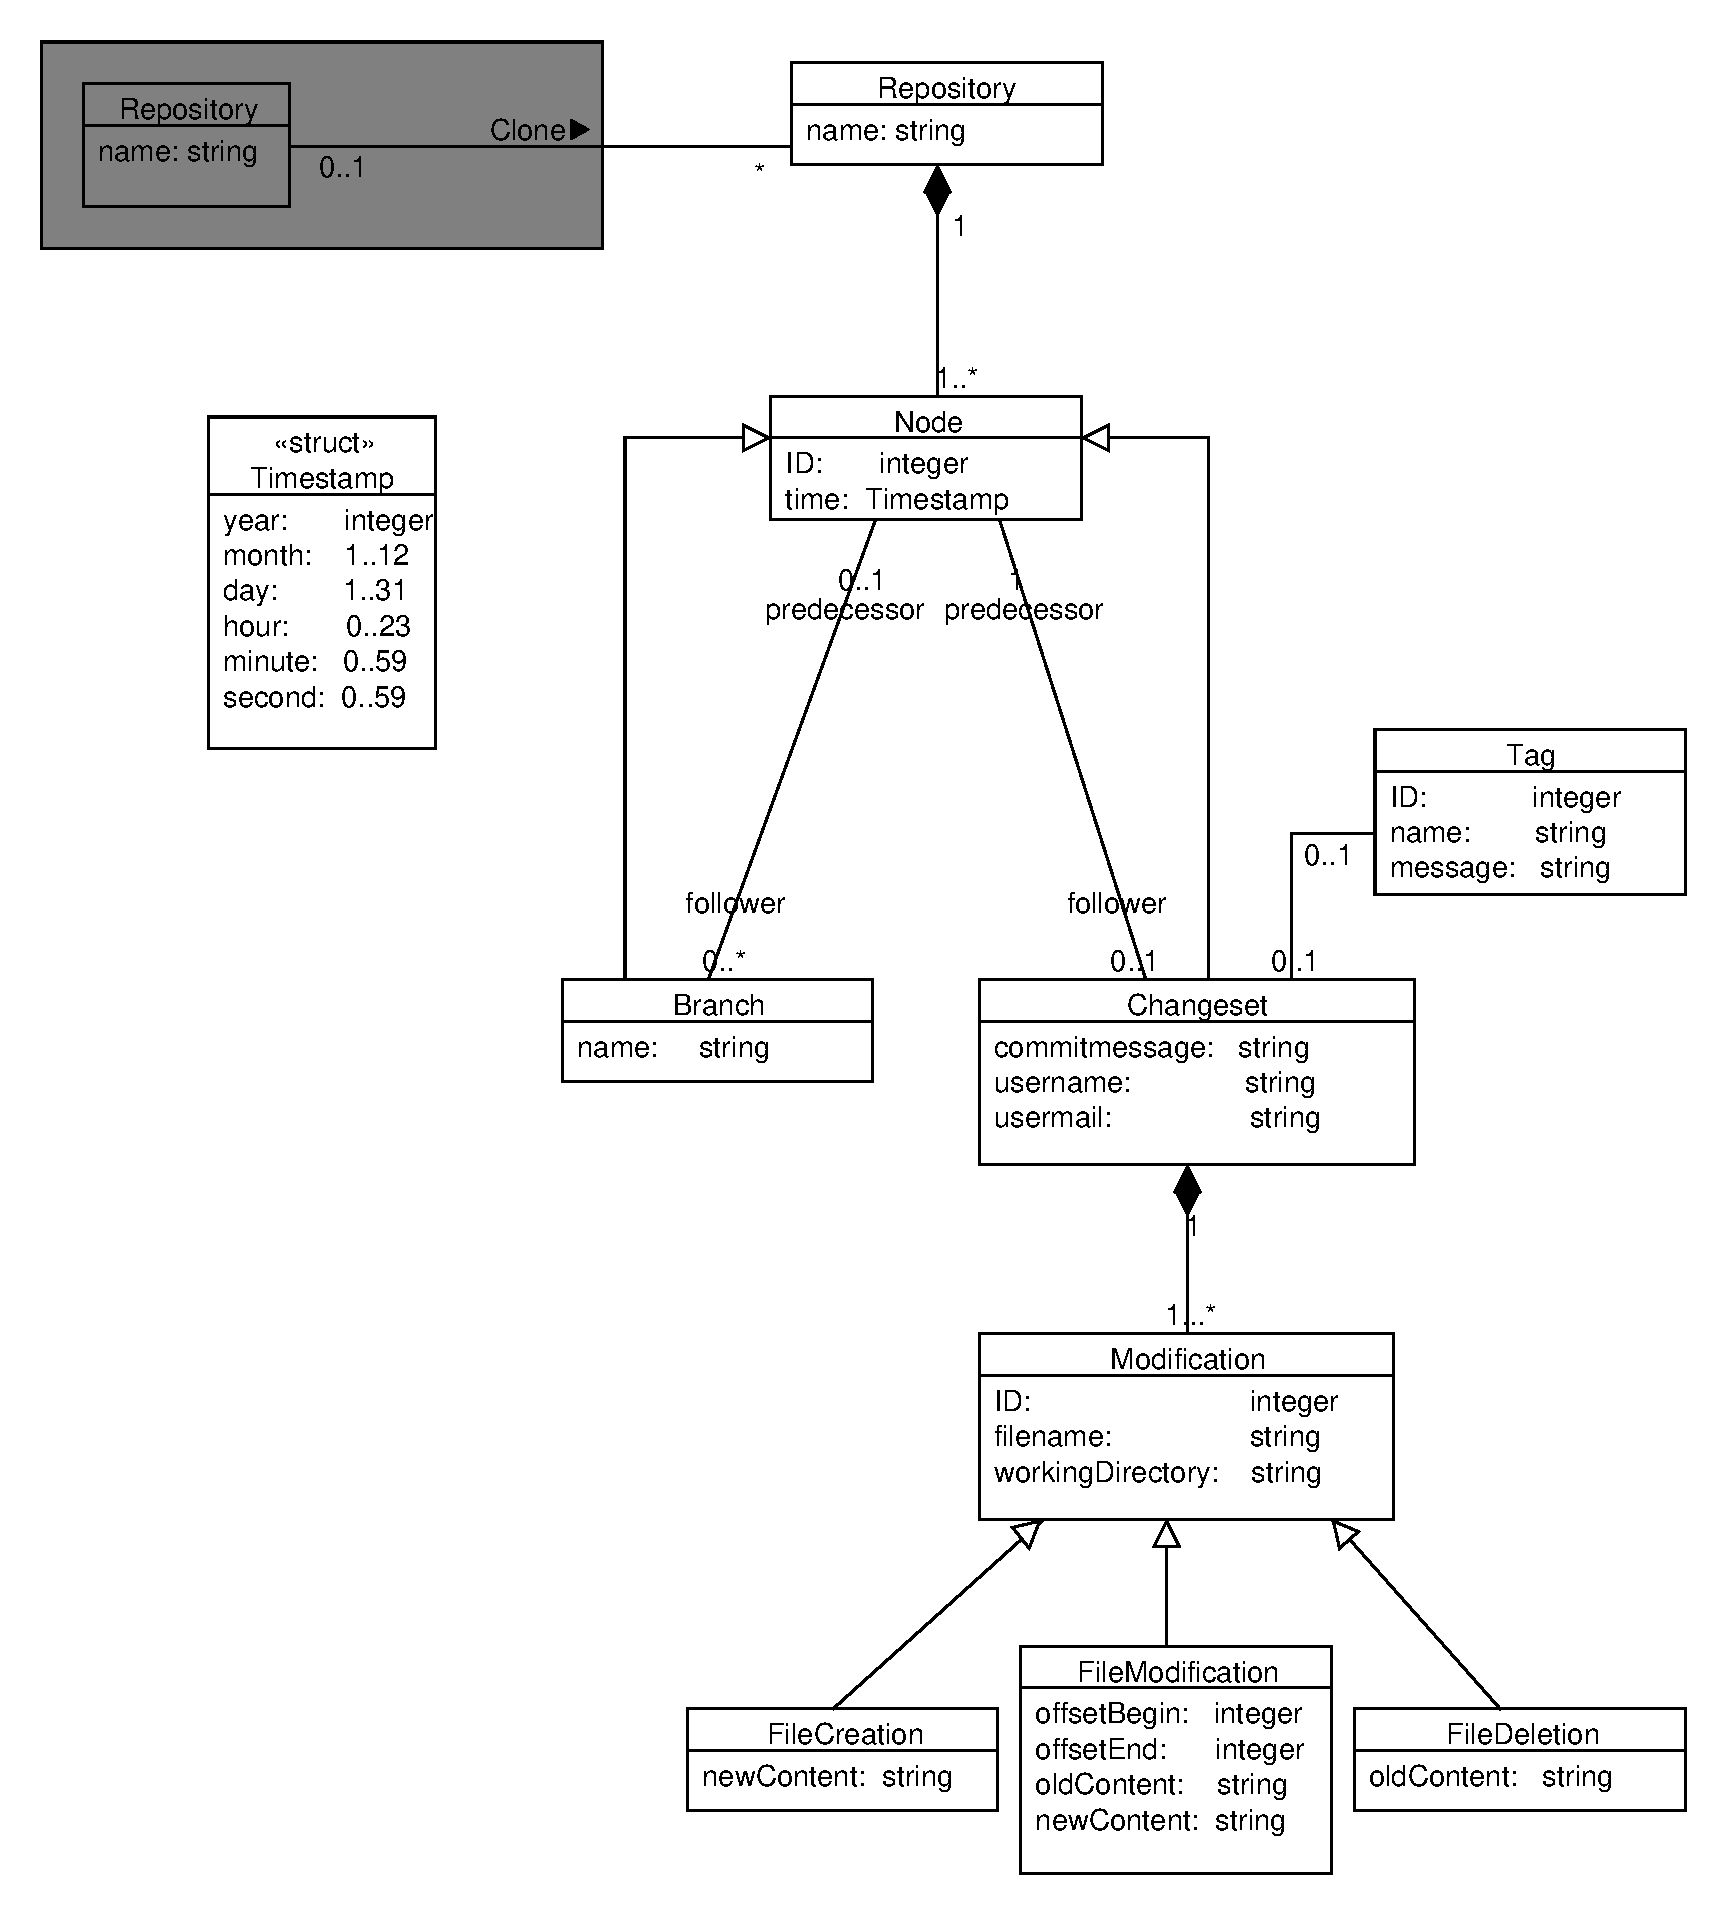
\includegraphics[width=\textwidth]{Domaenenmodell.pdf}\\
Die Abbildung stellt das Domänenmodell der Software GIT dar.\\\\

Das Repository ist die Hauptklasse unseres Modells. Es kann ein Repository auf einem Server existieren, von dem beliebig viele lokale Repositories geklont werden können (siehe \hyperlink{target}{Clone Repository} - Zustandsdiagramme). Zu jedem Repository gehören mindestens ein oder mehrere Branches und beliebig viele \gls{Changeset}s. Branches und Changesets sind Knoten. Changesets benötigen immer einen Vorgängerknoten somit gilt, dass ein Branch immer zuerst existieren muss. Auf einen Knoten können beliebig viele Branches folgen. Branches verzweigen also die History. Jedes Changeset beinhaltet mindestens eine Modifikation. Es gibt mehrere Arten von Modifikationen. Eine FileModification beschreibt eine zusammenhängende Textpassage (durch die Offsets definiert) in einer Datei die geändert wurde. Außerdem können Dateien erzeugt oder gelöscht werden. Wenn ein File verschoben wird, entspricht das intern der Löschung und Neuerzeugung des Files.

\newpage		
\subsection{Ausgewählte Zustandsdiagramme} \label{sec:zustandsd}

	Um das Verhalten eines Programms im laufenden Betrieb zu untersuchen, bedient man sich sogenannter \textbf{Zustandsdiagramme} \\
	Zustandsdiagramme bieten ein geeignetes Vokabular um das Ein- und Ausgabeverhalten eines Programms kompakt und präzise zu beschreiben.
	Da die Lebenszyklen der Objekte in Git komplex sind wurde hier ausgewählte Zustandsdiagramme dargestellt. \\

\underline{\textbf{\textsc{Push und Commit}}} \\
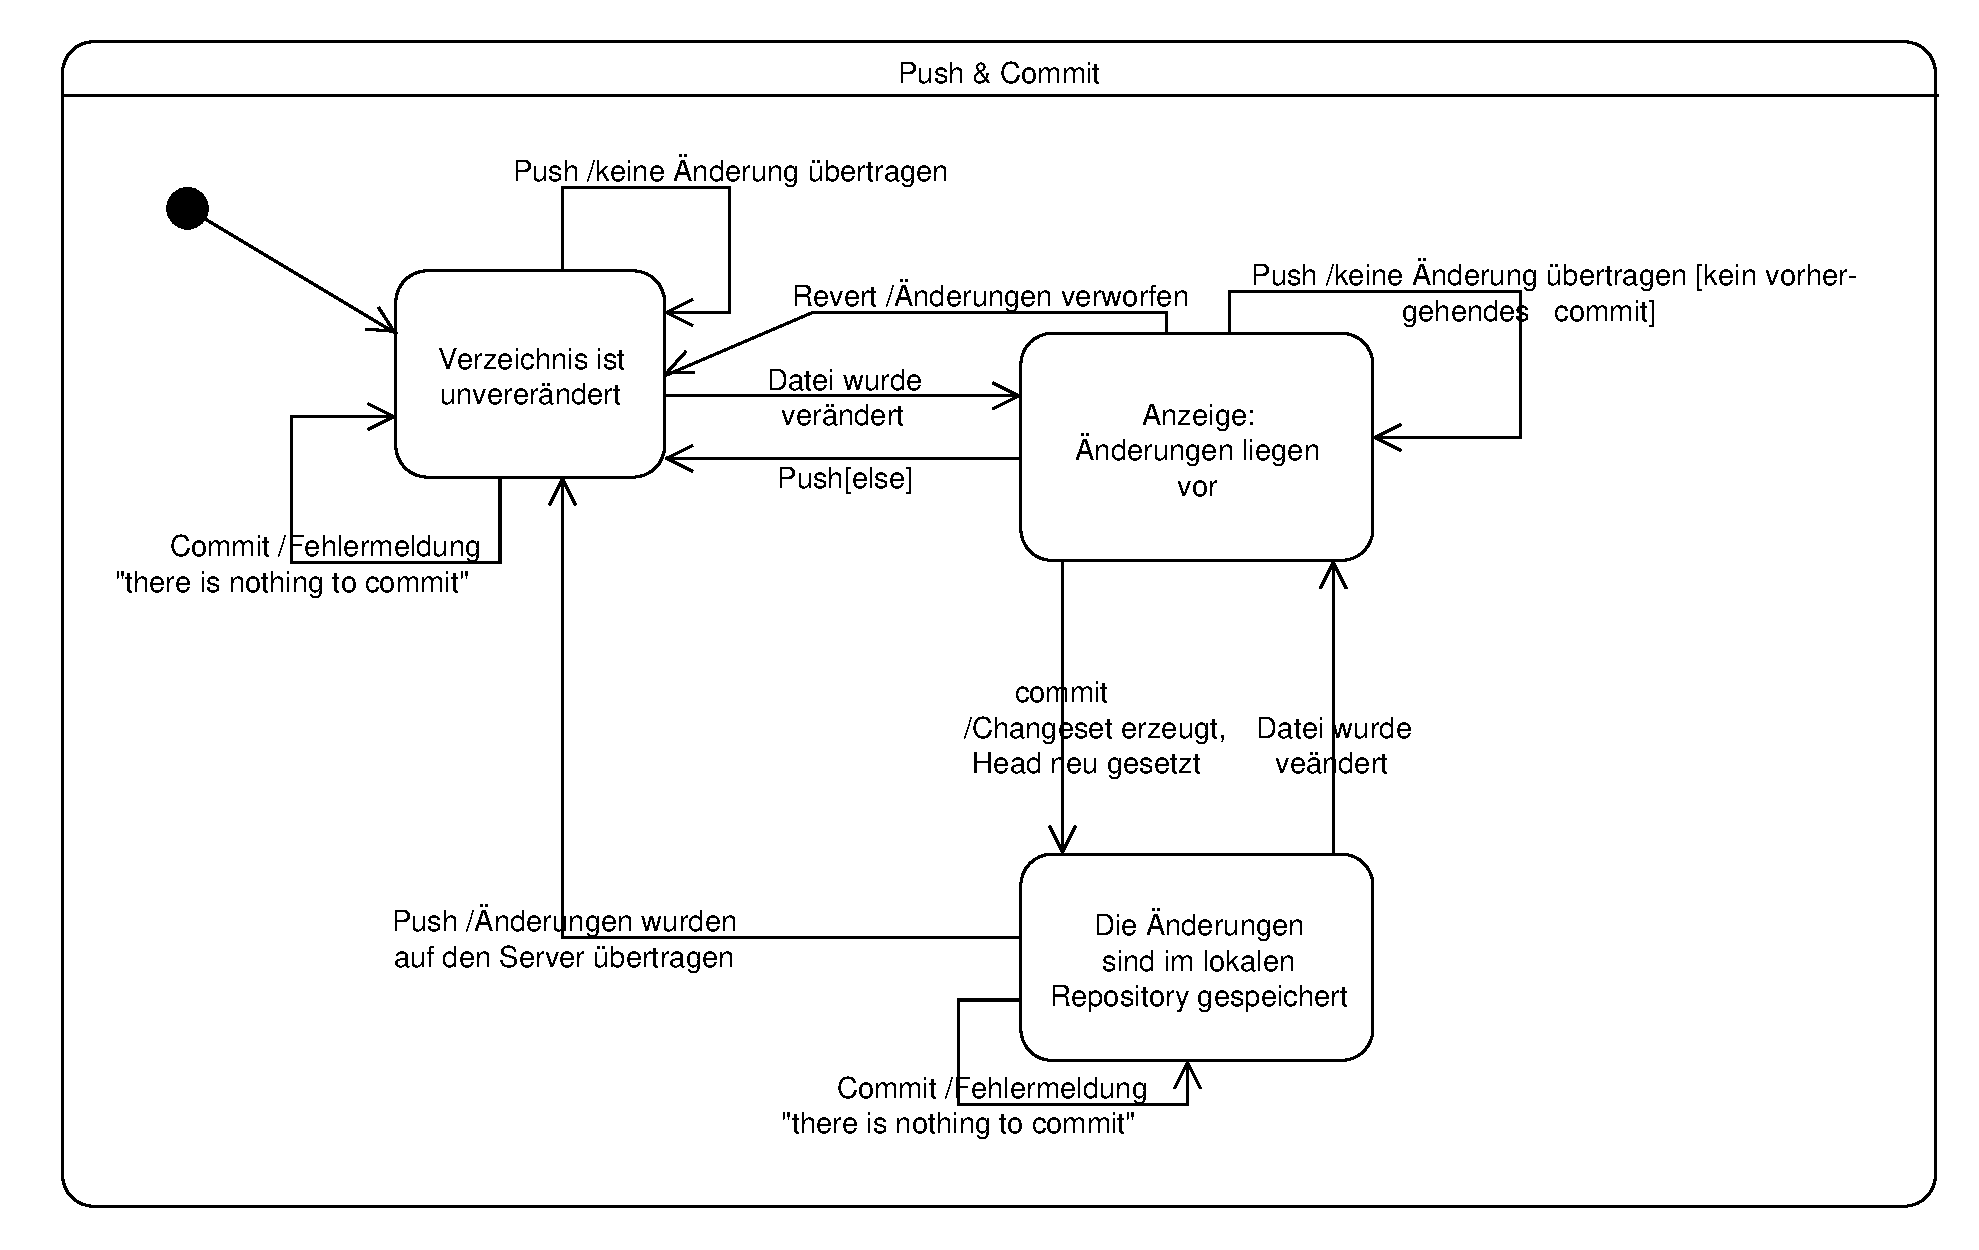
\includegraphics[width=\textwidth]{PuCo_Baar.pdf}\\\\
Die Möglichkeit zu commiten gibt es nur, wenn Änderungen vorliegen. Ansonsten wird eine Fehlermeldung ausgegeben, die den Nutzer darauf aufmerksam macht, dass es nichts zu commiten gibt.
Wurden Dateien oder Dokumente verändert, wird im SmartGit Fenster angezeigt, welche Dateien verändert wurden.\\
Der Nutzer hat in jedem Zustand die Möglichkeit, den Push-Button zu betätigen, allerdings mit unterschiedlichem Effekt:\\
Wurden die Änderungen noch nicht committed werden sie auch nicht auf den Server übertragen.
Es gibt nun den Fall, dass Änderungen vorgenommen und committed wurden, ohne das sie gepusht wurden.
Wenn der Nutzer nun weitere Änderung vornimmt, hat er die Möglichkeit die vorhergegangenen Änderungen auf den Server zu pushen, ohne dass die aktuellen Änderungen mit übernommen werden. 
\newpage	
\underline{\textbf{\textsc{\hypertarget{target}{Clone Repository}}}} \\
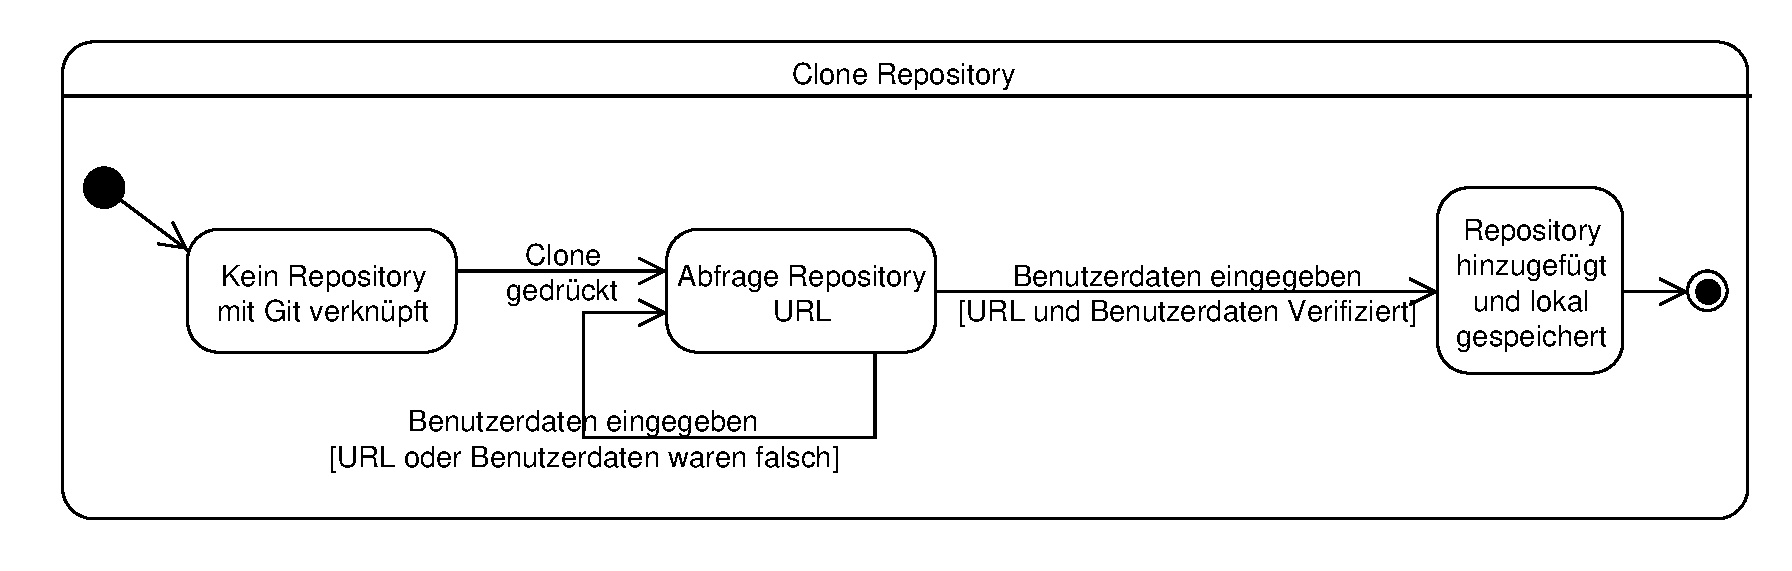
\includegraphics[width=\textwidth]{Clone.pdf}\\\\
Zu Beginn eines Projektes kann der Anwender ein existierendes Repository zu seinem Projekt hinzufügen.
Dafür benötigt er die genaue Web-Adresse eines bereits existierenden Repositorys. Diese wird dann vom System validiert. Bei falscher Eingabe gibt es eine Fehlermeldung und der Nutzer gelangt zurück in das Abfragemenü.
Bei erfolgreicher Anmeldung wird das Repository lokal auf dem Computer gespeichert. \\\\
Alternative kann auch ein lokales leeres Repository initialisiert werden.\\\\\\
\underline{\textbf{\textsc{Pull}}}\\
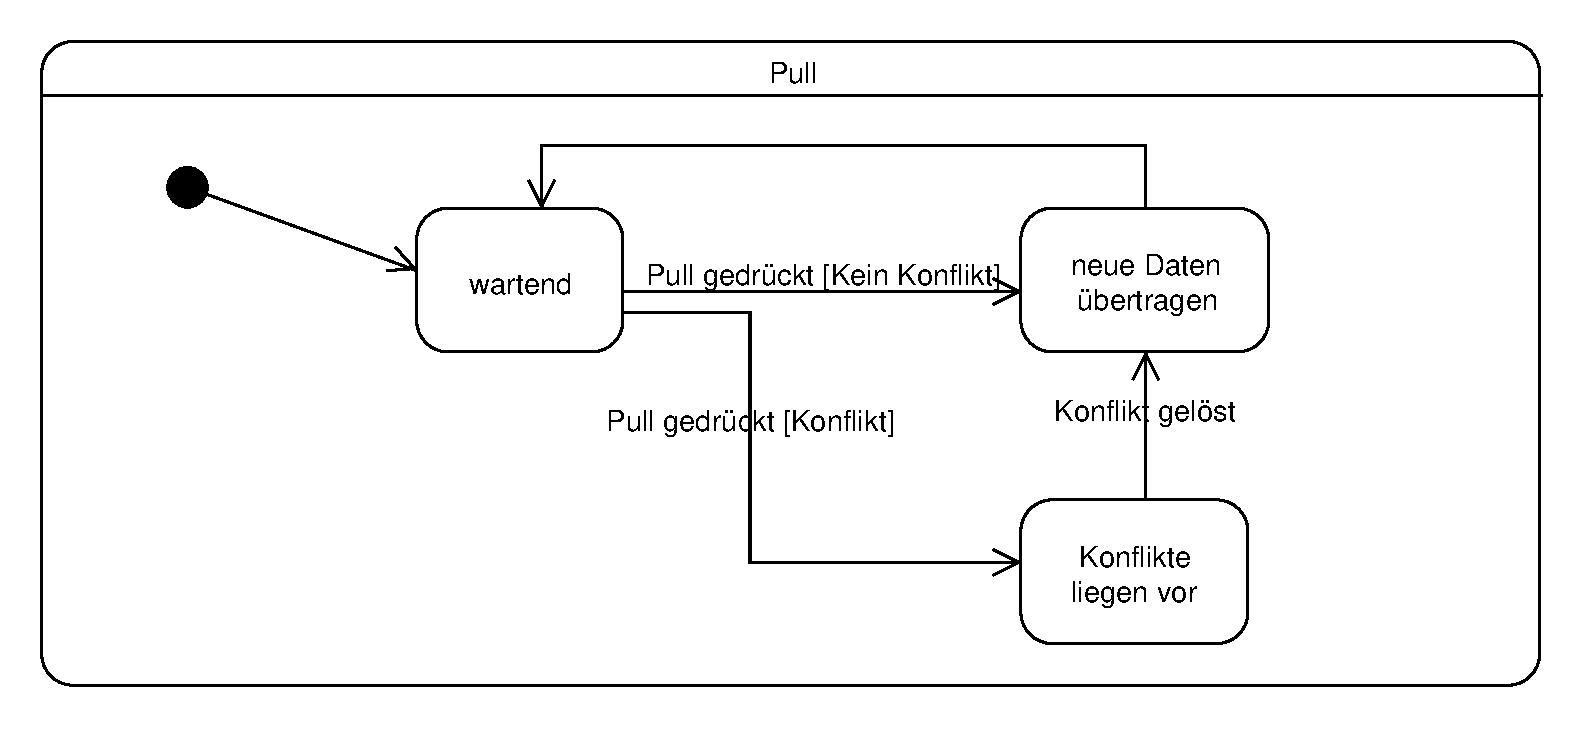
\includegraphics[width=\textwidth]{Pull.pdf}\\\\
Zu jedem vom Nutzer gewählten Zeitpunkt hat er die Möglichkeit, sein lokales Repository mit dem externen Repository abzugleichen. \\
Dafür wählt er die Option Pull, die alle seit dem letzten Abgleich veränderten Daten übernimmt.
Ein Konflikt tritt auf, wenn Änderungen an der gleichen Stelle vorgenommen wurden.
Der Nutzer muss dann den Konflikt lösen in dem er dem Programm sagt welche Änderung übernommen werden soll.

\newpage	
%---Glossar als subsection und "Glossar" einfügen------------------------------------------
\setglossarysection{subsection}
\printglossary[title={Glossar}, numberedsection]

%------------------------------------------------------------------------------------------

\newpage		
\section{\underline{Erfahrung aus der Teamarbeit}}

Zu Beginn unseres Projektes haben wir uns dazu entschieden GIT für die Versionsverwaltung und den Austausch zu nutzen. Da die üblichen Textverwaltungsprogramme ihren Inhalt nicht als Klartext speichern, welches eine Voraussetzung für GIT ist, haben wir uns dazu entschieden \LaTeX{} zu nutzen. Somit hat uns GIT beste Möglichkeiten geboten gemeinsam an dem Projekt zu arbeiten. Die Versionsverwaltung und das Austauschen der Daten ermöglichten uns auch in Zweiergruppen an den einzelnen Punkten zu arbeiten. Das gemeinschaftliche Zusammenfügen der Daten lief nicht immer problemlos, somit hatten wir die Möglichkeit uns intensiv mit der Software auseinander zu setzen. Wie bereits aus anderen Gruppenarbeiten zu erwarten lief die Teamarbeit problemlos ab. 
Die Teamarbeit lässt sich alles in allem als erfolgreich betrachten. Auch wenn es nicht immer einfach war ein gemeinsames Treffen zu koordinieren. 
\\\\

\section{\underline{Schlussbetrachtung}}
	
Zusammenfassend lässt sich sagen, dass diese Projektarbeit eine gute Möglichkeit war sich mit GIT und mit den Werkzeugen des Software Engineerings auseinander zu setzen. Es ist allerdings zu bedenken, dass man eine gewisse Einbearbeitungszeit benötigt um mit GIT umgehen zu können. Des Weiteren haben wir dieses Projekt dazu genutzt uns mit \LaTeX{} näher zu beschäftigen. Es hat uns fasziniert die Möglichkeiten von \LaTeX{} zu entdecken, auch wenn es hier und da einige Probleme gab.\\

\end{document}

